\documentclass{article}\usepackage[]{graphicx}\usepackage[]{color}
%% maxwidth is the original width if it is less than linewidth
%% otherwise use linewidth (to make sure the graphics do not exceed the margin)
\makeatletter
\def\maxwidth{ %
  \ifdim\Gin@nat@width>\linewidth
    \linewidth
  \else
    \Gin@nat@width
  \fi
}
\makeatother

\definecolor{fgcolor}{rgb}{0.251, 0.251, 0.282}
\newcommand{\hlnum}[1]{\textcolor[rgb]{0.125,0.125,1}{#1}}%
\newcommand{\hlstr}[1]{\textcolor[rgb]{0.125,0.125,1}{#1}}%
\newcommand{\hlcom}[1]{\textcolor[rgb]{1,0,0.753}{\textit{#1}}}%
\newcommand{\hlopt}[1]{\textcolor[rgb]{0.251,0.251,0.282}{#1}}%
\newcommand{\hlstd}[1]{\textcolor[rgb]{0.251,0.251,0.282}{#1}}%
\newcommand{\hlkwa}[1]{\textcolor[rgb]{0,0.533,0.345}{\textbf{#1}}}%
\newcommand{\hlkwb}[1]{\textcolor[rgb]{0.439,0.251,1}{\textbf{#1}}}%
\newcommand{\hlkwc}[1]{\textcolor[rgb]{0.529,0,0.184}{\textbf{#1}}}%
\newcommand{\hlkwd}[1]{\textcolor[rgb]{0.251,0.251,0.282}{\textbf{#1}}}%

\usepackage{framed}
\makeatletter
\newenvironment{kframe}{%
 \def\at@end@of@kframe{}%
 \ifinner\ifhmode%
  \def\at@end@of@kframe{\end{minipage}}%
  \begin{minipage}{\columnwidth}%
 \fi\fi%
 \def\FrameCommand##1{\hskip\@totalleftmargin \hskip-\fboxsep
 \colorbox{shadecolor}{##1}\hskip-\fboxsep
     % There is no \\@totalrightmargin, so:
     \hskip-\linewidth \hskip-\@totalleftmargin \hskip\columnwidth}%
 \MakeFramed {\advance\hsize-\width
   \@totalleftmargin\z@ \linewidth\hsize
   \@setminipage}}%
 {\par\unskip\endMakeFramed%
 \at@end@of@kframe}
\makeatother

\definecolor{shadecolor}{rgb}{.97, .97, .97}
\definecolor{messagecolor}{rgb}{0, 0, 0}
\definecolor{warningcolor}{rgb}{1, 0, 1}
\definecolor{errorcolor}{rgb}{1, 0, 0}
\newenvironment{knitrout}{}{} % an empty environment to be redefined in TeX

\usepackage{alltt}

% caracteres do portugues e formatacao tb 
\usepackage[utf8]{inputenc}
\usepackage[brazil]{babel}

% inclusao de referencias externas
\usepackage{hyperref}

\title{Exemplo F-DLM com dados artificiais}
\author{Rafael Barcellos}
\date{\today}
\IfFileExists{upquote.sty}{\usepackage{upquote}}{}

\begin{document}


\maketitle

\begin{abstract}
Este documento ilustra uma aplicação das funções que compõem o pacote \texttt{MScPack}. Todos os códigos do projeto se encontram em \href{https://github.com/rambs/MScPack}{github.com}
\end{abstract}

\section{Simulação dos dados artificiais}
Para simularmos dados artificiais do modelo linear dinâmico fatorial (F-DLM), basta utilizar a função \texttt{mdfDiscW.sim}. O código abaixo simula $T = 500$ observações de $q = 9$ variáveis.
\begin{knitrout}
\definecolor{shadecolor}{rgb}{0.973, 0.973, 0.973}\color{fgcolor}\begin{kframe}
\begin{verbatim}
TT = 500
set.seed(293874)
xDyn = 3 + cumsum(rnorm(TT, 0, 0.05))
plot(xDyn, type = "l")
\end{verbatim}
\end{kframe}\begin{figure}[]

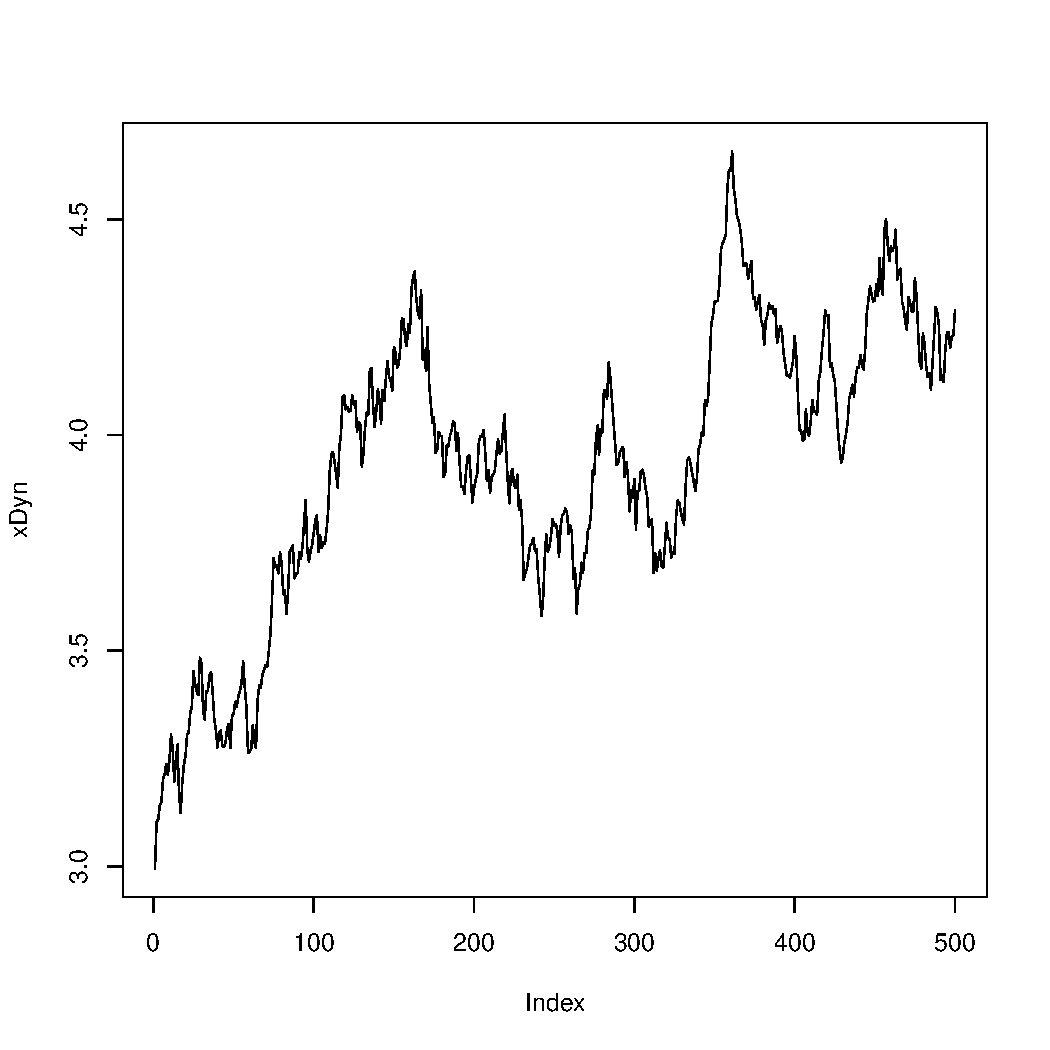
\includegraphics[width=\maxwidth]{figure/simExog} \caption[Exogenas geradas artificialmente]{Exogenas geradas artificialmente\label{fig:simExog}}
\end{figure}


\end{knitrout}


\begin{knitrout}
\definecolor{shadecolor}{rgb}{0.973, 0.973, 0.973}\color{fgcolor}\begin{kframe}
\begin{alltt}
\hlstd{xFix} \hlkwb{=} \hlkwd{rep}\hlstd{(}\hlnum{1}\hlstd{, TT)}
\hlstd{parmsFix} \hlkwb{=} \hlopt{-}\hlkwd{c}\hlstd{(}\hlnum{0.8}\hlstd{,} \hlnum{0.92}\hlstd{,} \hlnum{1.01}\hlstd{,} \hlnum{1.1}\hlstd{,} \hlnum{0.79}\hlstd{,} \hlnum{0.98}\hlstd{,} \hlnum{0.94}\hlstd{,} \hlnum{1.07}\hlstd{,} \hlnum{0.77}\hlstd{)}
\hlstd{q} \hlkwb{=} \hlkwd{length}\hlstd{(parmsFix)}
\hlstd{m0} \hlkwb{=} \hlkwd{rep}\hlstd{(}\hlnum{1}\hlstd{, q)}
\hlstd{C0} \hlkwb{=} \hlkwd{diag}\hlstd{(}\hlnum{0.01}\hlstd{, q)}
\hlstd{k} \hlkwb{=} \hlnum{3}
\hlstd{Lambda.lim} \hlkwb{=} \hlnum{0.1}
\hlkwd{set.seed}\hlstd{(}\hlnum{1928}\hlstd{)}
\hlstd{Lambda} \hlkwb{=} \hlkwd{array}\hlstd{(}\hlkwd{runif}\hlstd{(q} \hlopt{*} \hlstd{k,} \hlnum{0}\hlstd{, Lambda.lim),} \hlkwd{c}\hlstd{(q, k))}
\hlstd{Lambda[}\hlkwd{upper.tri}\hlstd{(Lambda)]} \hlkwb{=} \hlnum{0}
\hlkwd{diag}\hlstd{(Lambda)} \hlkwb{=} \hlkwd{c}\hlstd{(}\hlnum{0.99}\hlstd{,} \hlnum{0.95}\hlstd{,} \hlnum{0.9}\hlstd{)} \hlopt{*} \hlstd{Lambda.lim}
\hlstd{psi} \hlkwb{=} \hlkwd{c}\hlstd{(}\hlnum{0.02}\hlstd{,} \hlnum{0.19}\hlstd{,} \hlnum{0.36}\hlstd{,} \hlnum{0.02}\hlstd{,} \hlnum{0.02}\hlstd{,} \hlnum{0.19}\hlstd{,} \hlnum{0.19}\hlstd{,} \hlnum{0.36}\hlstd{,} \hlnum{0.36}\hlstd{)} \hlopt{*} \hlstd{Lambda.lim}\hlopt{/}\hlnum{10}
\hlstd{comunal} \hlkwb{=} \hlkwd{diag}\hlstd{(}\hlkwd{tcrossprod}\hlstd{(Lambda))}
\hlstd{comunal}\hlopt{/}\hlstd{(comunal} \hlopt{+} \hlstd{psi)}
\end{alltt}
\begin{verbatim}
## [1] 0.9800 0.8636 0.7999 0.9716 0.9629 0.9240 0.8618 0.7871 0.8340
\end{verbatim}
\end{kframe}
\end{knitrout}



\begin{knitrout}
\definecolor{shadecolor}{rgb}{0.973, 0.973, 0.973}\color{fgcolor}\begin{kframe}
\begin{alltt}
\hlkwd{library}\hlstd{(MScPack)}
\end{alltt}


{\ttfamily\noindent\itshape\color{messagecolor}{\#\# Loading required package: Rcpp}}

{\ttfamily\noindent\color{warningcolor}{\#\# Warning: package 'Rcpp' was built under R version 3.0.3}}

{\ttfamily\noindent\itshape\color{messagecolor}{\#\# Loading required package: RcppArmadillo}}

{\ttfamily\noindent\color{warningcolor}{\#\# Warning: package 'RcppArmadillo' was built under R version 3.0.3}}\begin{alltt}
\hlstd{mdfSim} \hlkwb{=} \hlkwd{mdfDiscW.sim}\hlstd{(xFix,} \hlkwd{array}\hlstd{(parmsFix,} \hlkwd{c}\hlstd{(}\hlnum{1}\hlstd{, q)), xDyn, m0, C0,} \hlnum{0.95}\hlstd{, Lambda,}
    \hlstd{psi,} \hlnum{90165}\hlstd{)}
\hlkwd{par}\hlstd{(}\hlkwc{mfrow} \hlstd{=} \hlkwd{c}\hlstd{(}\hlnum{3}\hlstd{,} \hlnum{3}\hlstd{),} \hlkwc{mar} \hlstd{=} \hlkwd{c}\hlstd{(}\hlnum{2.1}\hlstd{,} \hlnum{2.1}\hlstd{,} \hlnum{0.1}\hlstd{,} \hlnum{0.1}\hlstd{))}
\hlkwd{invisible}\hlstd{(}\hlkwd{apply}\hlstd{(mdfSim}\hlopt{$}\hlstd{y,} \hlnum{2}\hlstd{, plot,} \hlkwc{type} \hlstd{=} \hlstr{"l"}\hlstd{,} \hlkwc{bty} \hlstd{=} \hlstr{"l"}\hlstd{))}
\end{alltt}
\end{kframe}\begin{figure}[]

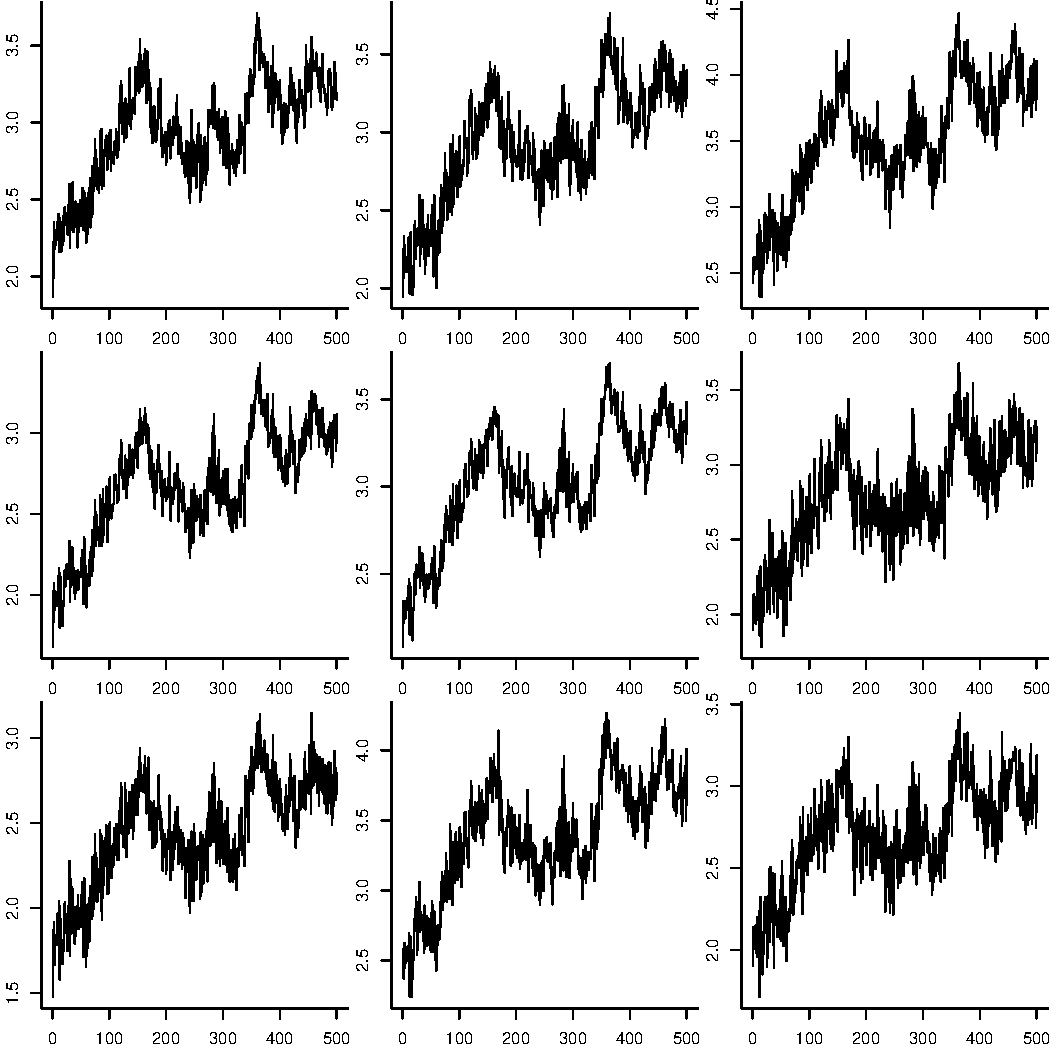
\includegraphics[width=\maxwidth]{figure/simData} \caption[F-DLM - Dados artificiais]{F-DLM - Dados artificiais\label{fig:simData}}
\end{figure}


\end{knitrout}


\begin{knitrout}
\definecolor{shadecolor}{rgb}{0.973, 0.973, 0.973}\color{fgcolor}\begin{kframe}
\begin{alltt}
\hlstd{modelo} \hlkwb{=} \hlkwd{list}\hlstd{(}\hlkwc{y} \hlstd{= mdfSim}\hlopt{$}\hlstd{y,} \hlkwc{xFixReg} \hlstd{= mdfSim}\hlopt{$}\hlstd{mod}\hlopt{$}\hlstd{xFixReg,} \hlkwc{xDynReg} \hlstd{= mdfSim}\hlopt{$}\hlstd{mod}\hlopt{$}\hlstd{xDynReg,}
    \hlkwc{nFactors} \hlstd{=} \hlkwd{ncol}\hlstd{(mdfSim}\hlopt{$}\hlstd{mod}\hlopt{$}\hlstd{Lambda),} \hlkwc{L0} \hlstd{=} \hlkwd{array}\hlstd{(}\hlnum{0}\hlstd{,} \hlkwd{dim}\hlstd{(mdfSim}\hlopt{$}\hlstd{mod}\hlopt{$}\hlstd{Lambda)),}
    \hlkwc{H0} \hlstd{=} \hlkwd{diag}\hlstd{(}\hlnum{100}\hlstd{,} \hlkwd{ncol}\hlstd{(mdfSim}\hlopt{$}\hlstd{mod}\hlopt{$}\hlstd{Lambda)),} \hlkwc{m0} \hlstd{=} \hlkwd{as.matrix}\hlstd{(mdfSim}\hlopt{$}\hlstd{mod}\hlopt{$}\hlstd{m0),}
    \hlkwc{C0} \hlstd{= mdfSim}\hlopt{$}\hlstd{mod}\hlopt{$}\hlstd{C0,} \hlkwc{b0} \hlstd{=} \hlkwd{array}\hlstd{(}\hlnum{0}\hlstd{,} \hlkwd{dim}\hlstd{(mdfSim}\hlopt{$}\hlstd{mod}\hlopt{$}\hlstd{parmsFixReg)),} \hlkwc{B0} \hlstd{=} \hlkwd{diag}\hlstd{(}\hlnum{1000}\hlstd{,}
        \hlkwd{nrow}\hlstd{(mdfSim}\hlopt{$}\hlstd{mod}\hlopt{$}\hlstd{parmsFixReg)),} \hlkwc{n0} \hlstd{=} \hlnum{1}\hlstd{,} \hlkwc{s0sq} \hlstd{=} \hlkwd{array}\hlstd{(mdfSim}\hlopt{$}\hlstd{mod}\hlopt{$}\hlstd{psi,}
        \hlkwd{c}\hlstd{(}\hlkwd{ncol}\hlstd{(mdfSim}\hlopt{$}\hlstd{y),} \hlnum{1}\hlstd{)),} \hlkwc{discW} \hlstd{= mdfSim}\hlopt{$}\hlstd{mod}\hlopt{$}\hlstd{discW)}
\hlstd{init.val} \hlkwb{=} \hlkwd{list}\hlstd{(}\hlkwc{Lambda} \hlstd{= mdfSim}\hlopt{$}\hlstd{mod}\hlopt{$}\hlstd{Lambda,} \hlkwc{psi} \hlstd{=} \hlkwd{as.matrix}\hlstd{(mdfSim}\hlopt{$}\hlstd{mod}\hlopt{$}\hlstd{psi),}
    \hlkwc{Beta} \hlstd{= mdfSim}\hlopt{$}\hlstd{mod}\hlopt{$}\hlstd{parmsFixReg)}
\end{alltt}
\end{kframe}
\end{knitrout}

\end{document}
